\documentclass[12pt, leqno]{article}
\usepackage{fancyhdr}
\usepackage[sort&compress]{natbib}
\usepackage[letterpaper=true,colorlinks=true,linkcolor=black]{hyperref}

\usepackage{amsfonts}
\usepackage{amsmath}
\usepackage{amssymb}
\usepackage{color}
\usepackage{tikz}
\usepackage{pgfplots}
\usepackage{listings}
%\usepackage{courier}
%\usepackage[utf8]{inputenc}
%\usepackage[russian]{babel}

\lstdefinelanguage{Julia}%
  {morekeywords={abstract,break,case,catch,const,continue,do,else,elseif,%
      end,export,false,for,function,immutable,import,importall,if,in,%
      macro,module,otherwise,quote,return,switch,true,try,type,typealias,%
      using,while},%
   sensitive=true,%
   alsoother={$},%
   morecomment=[l]\#,%
   morecomment=[n]{\#=}{=\#},%
   morestring=[s]{"}{"},%
   morestring=[m]{'}{'},%
}[keywords,comments,strings]%

\lstset{
  numbers=left,
  basicstyle=\ttfamily\footnotesize,
  numberstyle=\tiny\color{gray},
  stepnumber=1,
  numbersep=10pt,
}

\newcommand{\iu}{\ensuremath{\mathrm{i}}}
\newcommand{\bbR}{\mathbb{R}}
\newcommand{\bbC}{\mathbb{C}}
\newcommand{\calV}{\mathcal{V}}
\newcommand{\calE}{\mathcal{E}}
\newcommand{\calG}{\mathcal{G}}
\newcommand{\calW}{\mathcal{W}}
\newcommand{\calP}{\mathcal{P}}
\newcommand{\macheps}{\epsilon_{\mathrm{mach}}}
\newcommand{\matlab}{\textsc{Matlab}}
\newcommand{\uQ}{\underline{Q}}
\newcommand{\uR}{\underline{R}}

\newcommand{\ddiag}{\operatorname{diag}}
\newcommand{\fl}{\operatorname{fl}}
\newcommand{\nnz}{\operatorname{nnz}}
\newcommand{\tr}{\operatorname{tr}}
\renewcommand{\vec}{\operatorname{vec}}

\newcommand{\vertiii}[1]{{\left\vert\kern-0.25ex\left\vert\kern-0.25ex\left\vert #1
    \right\vert\kern-0.25ex\right\vert\kern-0.25ex\right\vert}}
\newcommand{\ip}[2]{\langle #1, #2 \rangle}
\newcommand{\ipx}[2]{\left\langle #1, #2 \right\rangle}
\newcommand{\order}[1]{O( #1 )}

\newcommand{\kron}{\otimes}


\newcommand{\hdr}[2]{
  \pagestyle{fancy}
  \lhead{Bindel, Fall 2020}
  \rhead{Numerical Analysis}
  \fancyfoot{}
  \begin{center}
    {\large{\bf HW for #1}} \\ (due: #2)
  \end{center}
  \lstset{language=Julia,columns=flexible}
}


\begin{document}
\hdr{2020-02-14}

\section{Cholesky}

So far, we have focused on the LU factorization for general
nonsymmetric matrices.  There is an alternate factorization
for the case where $A$ is {\em symmetric positive definite} (SPD),
i.e.
\begin{itemize}
\item $A = A^T$,
\item $x^T A x > 0$ for any $x \neq 0$.
\end{itemize}
For such a matrix, the {\em Cholesky factorization} is
\[
  A = LL^T \quad \mbox{ or } \quad A = R^T R
\]
where $L$ is a lower triangular matrix with positive diagonal and $R$
is an upper triangular matrix with positive diagonal ($R = L^T$).  The
Cholesky factor exists iff $A$ is positive definite; in fact, the
usual way to test numerically for positive definiteness is to attempt
a Cholesky factorization and see whether the algorithm succeeds or
fails.  And, unlike the LU factorization, the Cholesky factorization
is simply backward stable --- no appeal to pivot growth factors is required.

The Cholesky algorithm looks like Gaussian elimination.  As
with Gaussian elimination, we figure out what goes on
by block 2-by-2 factorization:
\[
\begin{bmatrix} A_{11} & A_{12} \\ A_{21} & A_{22} \end{bmatrix} =
\begin{bmatrix} L_{11} & 0 \\ L_{21} & L_{22} \end{bmatrix}
\begin{bmatrix} L_{11}^T & L_{21}^T \\ 0 & L_{22}^T \end{bmatrix} =
\begin{bmatrix}
  L_{11} L_{11}^T & L_{11} L_{21}^T \\
  L_{21} L_{11}^T & L_{21} L_{21}^T+ L_{22} L_{22}^T
\end{bmatrix}
\]
Working block-by-block, we have
\begin{align*}
  L_{11} L_{11}^T &= A_{11} \\
  L_{21} &= A_{21} L_{11}^{-T} \\
  L_{22} L_{22}^T &= A_{22} - L_{21} L_{21}^T
\end{align*}
That is, we factor the leading block, do a solve to get the
off-diagonal part, and then form and factor a Schur complement
system.

Note that the Schur complement
\[
  A_{22}-L_{21} L_{21}^T = A_{22} - A_{21} A_{11}^{-1} A_{12}
\]
is the same Schur complement that we see in Gaussian elimination
with partial pivoting; and, as in Gaussian elimination, we can
interpret the Schur complement as the inverse of a submatrix
of $A^{-1}$.  This is important because any principal submatrix of
an SPD matrix is SPD and inverses of SPD matrices are SPD, so
the Schur complements formed during Cholesky factorization remain
SPD.

In terms of basic MATLAB operations, Cholesky factorization looks like
\begin{lstlisting}
% Overwrite the lower triangular factor of A with L
for j = 1:n
  A(j,j) = sqrt(A(j,j));
  A(j+1:n,j) = A(j+1:n,j)/A(j,j);
  A(j+1:n,j+1:n) = A(j+1:n,j+1:n) - A(j+1:n,j)*A(j,j+1:n)';
end
\end{lstlisting}
This is very similar to the standard Gaussian elimination loop.
The only place where we might be concerned is that we could get
into trouble if we ever encountered a zero or negative diagonal
element; but the fact that the Schur complements remain SPD, together
with the fact that the diagonals of an SPD matrix are all positive,
suffices to guarantee this will never happen.

\section{Tricky tridiagonals}

Consider the tridiagonal matrix
\[
T = \begin{bmatrix}
  a_1 & b_1 \\
  c_2 & a_2 & b_2 \\
      & c_3 & a_3 & b_3 \\
      &     & \ddots & \ddots & \ddots \\
      &     &        & c_{n-1} & a_{n-1} & b_{n-1} \\
      &     &        &        & c_n     & a_n
  \end{bmatrix}
\]
What happens if we factor using Gaussian elimination?  We'll consider
first the case of no pivoting.  At the first step of elimination,
we subtract a multiple of the first row from the second row,
introducing a zero in the $(2,1)$ position.  Then we subtract a
multiple of the second row from the third row, and so on.
At each step, we only work with two rows of the matrix.  Let's write
the first two steps in pictures, assuming an implementation where
we are systematically overwriting the original matrix with lower
and upper triangular factors.  At each step, we color the entries
of the matrix that are transformed.  In the first step, we have
\[
  \begin{bmatrix}
  a_1 & b_1 \\
  c_2 & a_2 & b_2 \\
      & c_3 & a_3 & b_3 \\
      &     & \ddots & \ddots & \ddots \\
      &     &        & c_{n-1} & a_{n-1} & b_{n-1} \\
      &     &        &        & c_n     & a_n
  \end{bmatrix} \rightarrow
  \begin{bmatrix}
  a_1 & b_1 \\
  {\bf l_2} & {\bf \hat{a}_2} & b_2 \\
      & c_3 & a_3 & b_3 \\
      &     & \ddots & \ddots & \ddots \\
      &     &        & c_{n-1} & a_{n-1} & b_{n-1} \\
      &     &        &        & c_n     & a_n
  \end{bmatrix}
\]
At the next step, we have
\[
  \begin{bmatrix}
  a_1 & b_1 \\
  c_2 & a_2 & b_2 \\
      & c_3 & a_3 & b_3 \\
      &     & \ddots & \ddots & \ddots \\
      &     &        & c_{n-1} & a_{n-1} & b_{n-1} \\
      &     &        &        & c_n     & a_n
  \end{bmatrix} \rightarrow
  \begin{bmatrix}
  a_1 & b_1 \\
  l_2 & \hat{a}_2 & b_2 \\
      & {\bf l_3} & {\bf \hat{a}_3} & b_3 \\
      &     & \ddots & \ddots & \ddots \\
      &     &        & c_{n-1} & a_{n-1} & b_{n-1} \\
      &     &        &        & c_n     & a_n
  \end{bmatrix}
\]
At the end of the iteration, we have
\[
  \begin{bmatrix}
  a_1 & b_1 \\
  c_2 & a_2 & b_2 \\
      & \ddots & \ddots & \ddots \\
      &        & c_{n-1} & a_{n-1} & b_{n-1} \\
      &        &        & c_n     & a_n
  \end{bmatrix} =
  \begin{bmatrix}
  1 & \\
  l_2 & 1 &  \\
      & \ddots & \ddots & \\
      &        & l_{n-1} & 1 \\
      &        &        & l_n     & 1
  \end{bmatrix}
  \begin{bmatrix}
  a_1 & b_1 \\
      & \hat{a}_2 & b_2 \\
      &      & \ddots & \ddots \\
      &        &      & \hat{a}_{n-1} & b_{n-1} \\
      &        &        &     & \hat{a}_n
  \end{bmatrix}
\]

In code, we go from the standard Gaussian elimination loop
\begin{lstlisting}
% Overwrite A with L and U
for j = 1:n-1
  A(j+1:n,j) = A(j+1:n,j)/A(j,j);
  A(j+1:n,j+1:n) = A(j+1:n,j+1:n) - A(j+1:n,j)*A(j,j+1:n);
end
\end{lstlisting}
to the simplified loop
\begin{lstlisting}
% Overwrite T with L and U
for j = 1:n-1
  T(j+1,j) = T(j+1,j)/T(j,j);
  T(j+1,j+1) = T(j+1,j+1) - T(j+1,j)*T(j,j+1);
end
\end{lstlisting}
The former loop does $O(n^2)$ work per step, while the latter does
$O(1)$ work per step; that is, factoring a tridiagonal costs $O(n)$
work per time, not the $O(n^3)$ cost of factoring an ordinary matrix.

Of course, since most of the entries in a tridiagonal are zero,
we waste space by storing every entry explicitly, just as we waste
time if we use the general-purpose Gaussian elimination procedure.
In general, it is better to store only the nonzero entries of the
matrix.  For example, in the case of the tridiagonal matrix,
we might store the $a$, $b$, and $c$ coefficients as vectors,
in which case Gaussian elimination looks like
\begin{lstlisting}
% Overwrite a with the L entries, and b and c with the U entries
for j = 1:n-1
  a(j+1) = a(j+1)/b(j);
  b(j+1) = b(j+1)-a(j+1)*c(j);
end
\end{lstlisting}

We can similarly write $O(n)$ time routines for forward and backward
substitution with the (bidiagonal) triangular factors of $T$.

\section{Consider sparsity}

Tridiagonal matrices (and more generally banded matrices) belong to
a more general family of {\em sparse} matrices, or matrices in which
the vast majority of the entries are zero.

Sparse matrices are a bit different from dense matrices.  In a dense
matrix, we store the elements of the matrix in a fixed order.  There
is no need to specify that a value at a specific location in memory
corresponds to a particular matrix element; that information is
implicit.  For special sparse matrices, such as banded matrices, one
can again come up with storage formats that have this property.  But
in a general sparse matrix format, though we only store the nonzero
entries, we also have to store the location of those entries.  This
has several consequences.  One is that memory access for sparse matrix
computations is less regular than in the dense case, and so they run
at a lower flop rate than dense computations (though they typically do
far fewer flops than corresponding dense computations might, so it's
still a win).  Also, operations that are trivial in the dense case
become more complicated in the sparse case.  For example, adding two
dense matrices is easy, but adding two sparse matrices can be rather
complicated, depending on the data structure that is used to store
them.

The one operation on sparse matrices that is really simple is
matrix-vector multiplication.  This costs $O(\mathrm{nnz})$ time,
where nnz is the number of nonzeros in the matrix.  We will see that
we can build iterative solvers that just use this operation, but
that's a topic for another day.  For now, the question is: can we do
fast Gaussian elimination on sparse matrices?  The answer is yes,
but whether it's a good idea or not depends a lot on the matrix.
We turn to why this is the case in the next section.

\section{General sparse direct methods}

Suppose $A$ is a sparse matrix, and $PA = LU$.  Will $L$ and $U$ also
be sparse?  The answer depends in a somewhat complicated way on the
structure of the graph associated with the matrix $A$, the pivot
order, and the order in which variables are eliminated.  Except in
very special circumstances, there will generally be more nonzeros in
$L$ and $U$ than there are in $A$; these extra nonzeros are referred
to as {\em fill}.  There are two standard ideas for minimizing fill:
\begin{enumerate}
\item
  Apply a {\em fill-reducing ordering} to the variables; that is,
  use a factorization
  \[
    PAQ = LU,
  \]
  where $Q$ is a column permutation chosen to approximately minimize
  the fill in $L$ and $U$, and $P$ is the row permutation used for
  stability.

  The problem of finding an elimination order that minimizes fill is
  NP-hard, so it is hard to say that any ordering strategy is really
  optimal.  But there is canned software for some heuristic orderings
  that tend to work well in practice.  From a practical perspective,
  then, the important thing is to remember that a fill-reducing
  elimination order tends to be critical to using sparse Gaussian
  elimination in practice.
\item
  Relax the standard partial pivoting condition, choosing the row
  permutation $P$ to balance the desire for numerical stability
  against the desire to minimize fill.
\end{enumerate}

For the rest of this lecture, we will consider the simplified case of
{\em structurally} symmetric matrices and factorization without
pivoting (which is stable for diagonally dominant systems and positive
definite systems).

\section{Sparse matrices, graphs, and tree elimination}

Consider the following illustrative example of how factoring a sparse
matrix can lead to more or less dense factors depending on the order
of elimination.  Putting in $\times$ to indicate a nonzero element, we
have
\[
  \begin{bmatrix}
    \times & \times & \times & \times & \times \\
    \times & \times &        &        &        \\
    \times &        & \times &        &        \\
    \times &        &        & \times &        \\
    \times &        &        &        & \times
  \end{bmatrix} =
  \begin{bmatrix}
    \times &        &        &        &        \\
    \times & \times &        &        &        \\
    \times & \times & \times &        &        \\
    \times & \times & \times & \times &        \\
    \times & \times & \times & \times & \times
  \end{bmatrix}
  \begin{bmatrix}
    \times & \times & \times & \times & \times \\
           & \times & \times & \times & \times \\
           &        & \times & \times & \times \\
           &        &        & \times & \times \\
           &        &        &        & \times
  \end{bmatrix}.
\]
That is, $L$ and $U$ have many more nonzeros than $A$.
These nonzero locations that appear in $L$ and $U$ and not in $A$
are called {\em fill-in}.  On the other hand, if we cyclically
permute the rows and columns of $A$, we have
\[
  \begin{bmatrix}
    \times &        &        &        & \times \\
           & \times &        &        & \times \\
           &        & \times &        & \times \\
           &        &        & \times & \times \\
    \times & \times & \times & \times & \times
  \end{bmatrix} =
  \begin{bmatrix}
    \times &        &        &        & \\
           & \times &        &        & \\
           &        & \times &        & \\
           &        &        & \times & \\
    \times & \times & \times & \times & \times
  \end{bmatrix}
  \begin{bmatrix}
    \times &        &        &        & \times \\
           & \times &        &        & \times \\
           &        & \times &        & \times \\
           &        &        & \times & \times \\
           &        &        &        & \times
  \end{bmatrix}.
\]
That is, the factorization of $PAP^T$ has {\em no} fill-in.

A sparse matrix $A$ can be viewed as an {\em adjacency matrices}
for an associated graphs: make one node for each row,
and connect node $i$ to node $j$ if $A_{ij} \neq 0$.  The graphs
for the two ``arrow'' matrices above are:
\begin{center}
  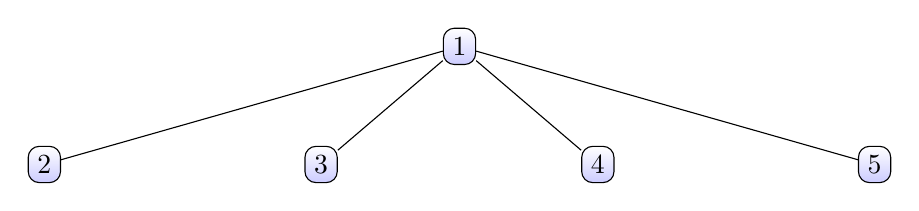
\begin{tikzpicture}[sibling distance=10em,
    every node/.style = {shape=rectangle, rounded corners,
    draw, align=center, top color=white, bottom color=blue!20}]
    \node {1}
      child { node {2} }
      child { node {3} }
      child { node {4} }
      child { node {5} };
  \end{tikzpicture}
  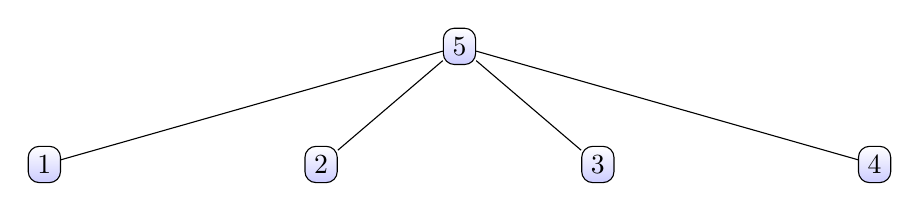
\begin{tikzpicture}[sibling distance=10em,
    every node/.style = {shape=rectangle, rounded corners,
    draw, align=center, top color=white, bottom color=blue!20}]
    \node {5}
      child { node {1} }
      child { node {2} }
      child { node {3} }
      child { node {4} };
  \end{tikzpicture}
\end{center}

These graphs of both our example matrices are {\em trees}, and they
differ only in how the nodes are labeled.  In the original matrix, the
root node is assigned the first label; in the second matrix, the root
node is labeled after all the children.  Clearly, the latter label
order is superior for Gaussian elimination.  This turns out to be a
general fact: if the graph for a (structurally symmetric) sparse
matrix $S$ is a tree, and if the labels are ordered so that each node
appears after any children it may have, then there is no fill-in: that
is, $L$ and $U$ have nonzeros only where $S$ has nonzeros.

Why should we have no fill when factoring a matrix for a tree ordered
from the leaves up?  To answer this, we think about what happens in the
first step of Gaussian elimination.  Our original matrix has the form
\[
  S = \begin{bmatrix} \alpha & w^T \\ v & S_{22} \end{bmatrix}
\]
The first row of $U$ is identical to the first row of $S$,
and the first column of $L$ has the same nonzero structure
as the first column of $A$, so we are fine there.
The only question is about the nonzero structure of the Schur
complement $S_{22}-vw^T/\alpha$.  Note that the update $vw^T/\alpha$
has nonzeros only where $v_i$ and $w_j$ are both nonzero --- that is,
only when nodes $i$ and $j$ are both connected to node $1$.  But node
1 is a leaf node; the only thing it connects to is its parent!  So if
$p$ is the index of the parent of node 1 in the tree, then we only
change the $(p,p)$ entry of the trailing submatrix during the update
--- and we assume that entry is already nonzero.  Thus, the graph
associated with the Schur complement is the same as the graph of the
original matrix, but with one leaf trimmed off.

\section{Nested dissection}

Tree-structured matrices are marvelous because we can do everything in
$O(n)$ time: we process the tree from the leaves to the root in order
to compute $L$ and $U$, then recurse from the root to the leaves in
order to do back substitution with $U$, and then go back from the
leaves to the root in order to do forward substitution with $L$.
Sadly, many of the graphs we encounter in practice do not look like trees.
However, we can often profitably think of clustering nodes so that we get
a {\em block} structure associated with a tree.

For illustrative purposes, let us consider Gaussian elimination on a
matrix whose graph is a regular $n \times n$ mesh.  Such a matrix
might arise, for example, if we were solving Poisson's equation using
a standard five-point stencil to discretize the Laplacian operator.
We then think of cutting the mesh in half by removing a set of
separator nodes, cutting the halves in half, and so forth.  This
yields a block structure of a tree consisting of a root (the separator
nodes) and two children (the blocks on either side of the separator).
We can now dissect each of the sub-blocks with a smaller separator,
and continue on in this fashion until we have cut the mesh into blocks
containing only a few nodes each.  Figure~\ref{fig1} illustrates the
first two steps in this process of {\em nested dissection}.

\begin{figure}
\begin{center}
\input{fig/ndfig.pdf_t}
\[
  S =
  \begin{bmatrix}
    S_{AA} &        & {\color[rgb]{0,0,1}S_{AC}} &      &        &       & {\color[rgb]{1,0,0}S_{AG}} \\
           & S_{BB} & {\color[rgb]{0,0,1}S_{BC}} &      &        &       & {\color[rgb]{1,0,0}S_{BG}} \\
    {\color[rgb]{0,0,1}S_{CA}} & {\color[rgb]{0,0,1}S_{CB}} & {\color[rgb]{0,0,1} S_{CC}} &       &        &       & {\color[rgb]{1,0,0}S_{CG}} \\
           &       &       & S_{DD} &        & {\color[rgb]{0,0,1}S_{DF}} & {\color[rgb]{1,0,0}S_{DG}} \\
           &       &       &       & S_{EE} & {\color[rgb]{0,0,1}S_{EF}} & {\color[rgb]{1,0,0}S_{EG}} \\
           &       &       & {\color[rgb]{0,0,1}S_{FD}} & {\color[rgb]{0,0,1}S_{FE}} & {\color[rgb]{0,0,1}S_{FF}} & {\color[rgb]{1,0,0}S_{FG}} \\
    {\color[rgb]{1,0,0}S_{GA}} & {\color[rgb]{1,0,0}S_{GB}} & {\color[rgb]{1,0,0}S_{GC}} & {\color[rgb]{1,0,0}S_{GD}} & {\color[rgb]{1,0,0}S_{GE}} & {\color[rgb]{1,0,0}S_{GF}} & {\color[rgb]{1,0,0}S_{GG}}
  \end{bmatrix}
\]
\end{center}
\caption{Nested dissection on a square mesh.  We first cut the graph in half
         with the red separator $G$, then further dissect the halves with the
         blue separators $C$ and $F$.  Nodes in $A$, $B$, $D$, and $F$ are only
         connected through these separator nodes, which is reflected in the
         sparsity pattern of the adjacency matrix $S$ when it is ordered so that
         separators appear after the things they separate.}
\label{fig1}
\end{figure}

We can get a lower bound on the cost of the factorization by figuring
out the cost of factoring the Schur complement associated with $G$,
$C$, $F$, etc.  After we eliminate everything except the nodes
associated with $G$, we pay about $2n^3/3$ flops to factor the
remaining (dense) $n$-by-$n$ Schur complement matrix $G$.  Similarly,
we pay about $2(n/2)^3/3$ time to factor the dense $(n/2)$-by-$(n/2)$
complements associated with the separators $C$ and $F$.  Eliminating
all four separators then costs a total of $\approx 10n^3/12$ flops.
Now, think of applying nested dissection to blocks $A$, $B$, $D$, and
$E$; eliminating the Shur complements associated with separators
inside each of these blocks will take about $5(n/2)^3/6$ flops; all
four together cost a total of $4 ( 5(n/2)^3/6 )= (1/2)
(5n^3/6)$ flops to factor.  If we keep recursing, we find that the
cost of factoring Schur complements associated with all the separators
looks like
\[
  \frac{5}{6} n^3 \left( 1 + \frac{1}{2} + \frac{1}{4} + \ldots \right)
  \approx \frac{5}{3}n^3.
\]
It turns out that forming each Schur complement is asymptotically not
more expensive than eliminating it, so that the overall cost of doing
nested dissection on an $n \times n$ mesh with $N = n^2$ unknown is also
$O(n^3) = O(N^{1.5})$.  It also turns out that the fill-in is
$O(N \log N)$\footnote{
  The explanation of why is not so hard, at least for regular 2D meshes,
  but it requires more drawing than I feel like at the moment.  The paper
  ``Nested Dissection of a Regular Finite Element Mesh'' by Alan George
  (SIAM J. Numer. Anal. 10(2), April 1973) gives a fairly readable explanation
  for the curious.
}.

Now think about doing the same thing with a three-dimensional mesh.
In this case, the top-level separators for an $n \times n \times n$ mesh
with $N = n^3$ unknowns would involve $n^2$ unknowns, and we would take
$O(n^6) = O(N^2)$ time to do the elimination, and $O(N^{4/3})$ fill.
This relatively poor scaling explains why sparse direct methods are attractive
for solving 2D PDEs, but are less popular for 3D problems.

\section{E pluribus unum}

% One problem vs many
% - Multiple right hand sides
% - Small changes in the matrix
% - Low rank changes in the matrix
% - Bigger changes

So far, we have described a few ideas about how to perform Gaussian
elimination for linear systems.  But you might find yourself asking a
reasonable --- if a bit lazy --- question: ``why bother?''  After all,
the MATLAB backslash operator is a marvelous invention, and the simple
expression
\begin{lstlisting}
  x = A\b;
\end{lstlisting}
mostly ``does the right thing'' for a variety of types of matrices.
If $A$ is square and dense, this line causes MATLAB to factor the
matrix $A$ using Gaussian elimination, then carry out forward and
backward substitution.  If $A$ is triangular, MATLAB detects that and
just does forward or backward substitution without a factorization
step.  If $A$ is a sparse matrix, MATLAB uses the UMFPACK sparse LU
package, including applying a reasonable column permutation.  If
MATLAB can do all this automatically for you, why do you need to know
the details?

There's a deeper answer to this question than the superficial
``because you're taking a numerical methods class.''  It even
goes beyond needing to understand things like when a sparse system
is best solved by a direct method vs.~an iteration.  One very
important reason to understand the factorizations that are being
computed behind the scenes is that those factorizations can be
{\em reused} when you are solving more than one linear system at a go.
And solving more than one problem at a time, as it turns out, is often
what we want to do.

\subsection{Multiple right hand sides}

The simplest case of solving multiple problems is when the matrix
is fixed, but there are several right hand sides.  That is,
we want to solve
\[
  A x^{(k)} = b^{(k)}
\]
for $k = 1, \ldots, m$.  In the simple case where all the right hand
sides are known in advance, we can still accomplish this by using
the magic of MATLAB's backslash:
\begin{lstlisting}
  X = A\B;
\end{lstlisting}
But in some cases, we might not know the $k$th right hand side until
we have learned the answer to the $k-1$th question.  For example,
suppose we wanted to run the iterative refinement process
\[
  x^{(k+1)} = x^{(k)} + \hat{A}^{-1} (b-Ax^{(k)})
\]
that was mentioned in a previous lecture.  In MATLAB, if we had
already computed the factorization
\begin{lstlisting}
  [L,U,P] = lu(A);
\end{lstlisting}
we might run the iteration
\begin{lstlisting}
  x = U\(L\(P*b));
  for k = 1:niter
    r = b-A*x;
    x = x + U\(L\(P*r));
  end
\end{lstlisting}
Note that we {\em never} form the inverse of $A$, explicitly or implicitly.
Rather, we apply $A^{-1}$ to vectors through triangular solves involving
the factors computed through Gaussian elimination.  Using only
triangular solves is good for performance (we take $O(n^2)$ time per
solve after the original factorization, rather than $O(n^3)$ time);
and it is good for numerical stability.

The admonition against inverses sometimes causes a certain amount of
confusion, and it bears repeating: {\em we want to only do
  permutations and triangular solves} applied to vectors.
Specifically, in MATLAB, we have
\begin{lstlisting}
  % Generally good
  x = U\(L\(P*b));

  % Generally bad
  x = inv(A)*b;     % Code that calls 'inv' deserves skepticism
  x = U\(L\(P'\b)); % Silly, since P^{-%} = P
  x = U\L\P*b;      % Order of operations means we form U\L!
  x = (U\(L\P)*b;   % U\(L\P) is an explicit inverse
\end{lstlisting}

\newpage
\section{Problems to ponder}

\begin{enumerate}
\item
  An SPD matrix always can be written $A = Q \Lambda Q^T$ where
  $\Lambda$ is a diagonal matrix with positive entries and $Q$ is
  an orthogonal matrix.  Show that $A^{-1}$ has a similar
  factorization, and therefore must also be SPD.
\item
  Argue that a principal submatrix of an SPD matrix must be SPD;
  for example, if
  \[
    A = \begin{bmatrix} A_{11} & A_{21}^T \\ A_{21} & A_{22} \end{bmatrix}
  \]
  is SPD, then so are $A_{11}$ and $A_{22}$.
\item
  If $A = LL^T$ is SPD, argue that
  $\|x\|_A^2 \equiv x^T A x = \|L^T x\|^2$.
\item
  Suppose $A$ is an SPD tridiagonal with diagonal entries
  $\alpha_{1}, \ldots, \alpha_n$ and off-diagonal entries
  $\beta_1, \ldots, \beta_{n-1}$.  Write a MATLAB loop that converts
  the vectors {\tt alpha} and {\tt beta} into corresponding
  coefficient vectors for a bidiagonal Cholesky factor of $A$.
\end{enumerate}

\end{document}
